\documentclass[12pt,a4paper]{article}

%--------------------------------
% PAQUETES
%--------------------------------
\usepackage[spanish]{babel}
\usepackage[utf8]{inputenc}
\usepackage[T1]{fontenc}
\usepackage{geometry}
\usepackage{graphicx}
\usepackage{float}
\usepackage{amsmath}
\usepackage{pdfpages}
\usepackage[colorlinks=true, linkcolor=blue, urlcolor=blue]{hyperref}

\geometry{margin=2.5cm}

%--------------------------------
% DATOS DEL INFORME (COMPLETAR)
%--------------------------------

%--------------------------------
\begin{document}

\pagenumbering{gobble}

%--------------------------------
% PORTADA
%--------------------------------
\begin{titlepage}
    \centering

    {\scshape\LARGE Universidad Tecnológica Nacional \par}
    \vspace{0.3cm}
    {\scshape\Large Facultad Regional Córdoba \par}
    \vspace{1.5cm}

    {\scshape\Large Técnicas Digitales I \par}
    \vspace{2cm}

    {\Huge\bfseries Trabajo Práctico N°0 \par}
    \vspace{0.5cm}
    {\LARGE MiniLab \par}

    \vspace{2cm}

    \begin{flushleft}
    \textbf{Integrantes:} \\
    Alejos Gamarra, Antony Jeanpol --- 413820 \\
    Cortesini Perez, Luciano Tomas  --- 402719 \\
    Moyano, Pablo Gabriel  --- 403337 \\

    \vspace{0.5cm}

    \textbf{Curso:} 3R\_3 \\
    \textbf{Grupo:} 03 \\
    \textbf{Docente:} Ing. Florencia Belén Molla \\
    \textbf{Año:} 2026 \\
    \end{flushleft}

    \vfill

\end{titlepage}
\thispagestyle{empty}

\clearpage
\pagenumbering{arabic}

\vspace{1cm}

\tableofcontents
\newpage

%--------------------------------
\section{Introducción}
%--------------------------------

%\textit{Describir brevemente el objetivo del trabajo práctico y para qué se construye el MiniLab.}

En el presente trabajo práctico se propone la construcción de un mini laboratorio
portátil (MiniLab), el cual será utilizado a lo largo de la materia Técnicas Digitales I
(TD1).
El objetivo principal de este dispositivo es proporcionar a cada estudiante una herramienta
práctica que le permita experimentar, analizar y verificar el funcionamiento de
circuitos digitales básicos.
El MiniLab está diseñado para facilitar el aprendizaje mediante la implementación
de entradas y salidas digitales, indicadores visuales mediante LEDs, y una fuente de
alimentación regulada. De manera opcional, se incorpora un generador de señal basado
en un temporizador 555, permitiendo ampliar las experiencias prácticas.
Este enfoque busca no solo reforzar los conceptos teóricos, sino también desarrollar
habilidades en el uso de instrumentos y herramientas propias del ámbito electrónico.

\vspace{0.5cm}

%--------------------------------
\section{Objetivos}
%--------------------------------

%\textit{Indicar qué se busca lograr con este trabajo (ej: construir el MiniLab, comprender su funcionamiento, etc.).}
\subsection{Objetivo General}
Diseñar y construir un mini laboratorio portátil (MiniLab) que permita realizar prácticas de electrónica digital de
manera autónoma, facilitando la experimentación y comprensión de los conceptos fundamentales de la materia.

\subsection{Objetivos específicos}

\begin{itemize}
    \item Construir un dispositivo que disponga de entradas y salidas digitales para la prueba
        de circuitos lógicos
    \item Implementar indicadores visuales mediante LEDs para representar estados lógicos.
    \item Incorporar una fuente de alimentación regulada de 5V para el funcionamiento de
        los circuitos.
    \item Comprender el funcionamiento y uso de herramientas básicas de laboratorio, tales
        como multímetro, pinza, alicate y soldador.
    \item Desarrollar habilidades prácticas en el armado, conexión y verificación de circuitos
        electrónicos.
    \item (Opcional) Implementar un generador de señal cuadrada mediante un temporizador
        555, con frecuencia variable
\end{itemize}   

\section{Requerimientos del sistema}
El MiniLab deberá cumplir con las siguientes características funcionales:

\begin{itemize}
    \item \textbf{Salidas digitales:}
        \begin{itemize}
            \item El sistema deberá contar con 6 salidas digitales.
            \item El nivel lógico bajo (“0”) corresponderá a 0V.
            \item El nivel lógico alto (“1”) corresponderá a 5V.
        \end{itemize}
    \item \textbf{Entradas digitales con indicación luminosa:}
        \begin{itemize}
            \item Se deberán implementar 6 entradas para conexión mediante punta de prueba.
            \item Cada entrada deberá contar con un LED indicador de estado: 
            \begin{itemize}
                \item LED apagado: lógico “0”
                \item LED encendido: lógico “1”
            \end{itemize}
        \end{itemize}
    \item \textbf{Generador de señal (opcional):}
        \begin{itemize}
            \item El sistema podrá incluir una salida de señal de onda cuadrada.
            \item La frecuencia deberá ser ajustable mediante un potenciómetro.
            \item Rango de frecuencia: 1 Hz a 1 kHz
        \end{itemize}
    \item \textbf{Fuente de alimentación:}
        \begin{itemize}
            \item El sistema deberá contar con una fuente regulada de 5V.
            \item La alimentación podrá realizarse mediante:
                \begin{itemize}
                    \item Red eléctrica (220V).
                    \item Batería de 9V (fuente auxiliar).
                \end{itemize}
        \end{itemize}
    \item \textbf{Placas de prototipado:}
        \begin{itemize}
            \item Se deberán incluir placas tipo protoboard para el armado de circuitos.
            \item Cantidad recomendada: 2 protoboards de 830 puntos.
        \end{itemize}
    \item \textbf{Herramientas de laboratorio:}
        \begin{itemize}
            \item El sistema deberá estar contenido en un gabinete o caja.
            \item El diseño deberá permitir su transporte y protección de los componentes.
        \end{itemize}
\end{itemize}

%--------------------------------
\section{Desarrollo}
%--------------------------------

\subsection{Descripción del sistema}

%\textit{Explicar cómo está compuesto el MiniLab (entradas, salidas, fuente, etc.).}
El MiniLab está compuesto por 4 bloques funcionales principales:

\subsubsection{Bloque de Fuente de Alimentación}
Este bloque proporciona una fuente de alimentación regulada de 5V, destinada a alimentar al resto de los
componentes del MiniLab como los circuitos que se deseen probar.
El regulador utilizado es un LM7805, el cual garantiza una salida estable de 5V a partir de una tensión de entrada de entre 7V y 35V.
Ademas, se incluyó un LED indicador que muestra el estado de la alimentación, encendiéndose cuando el sistema está energizado.

\begin{figure}[H]
    \centering
    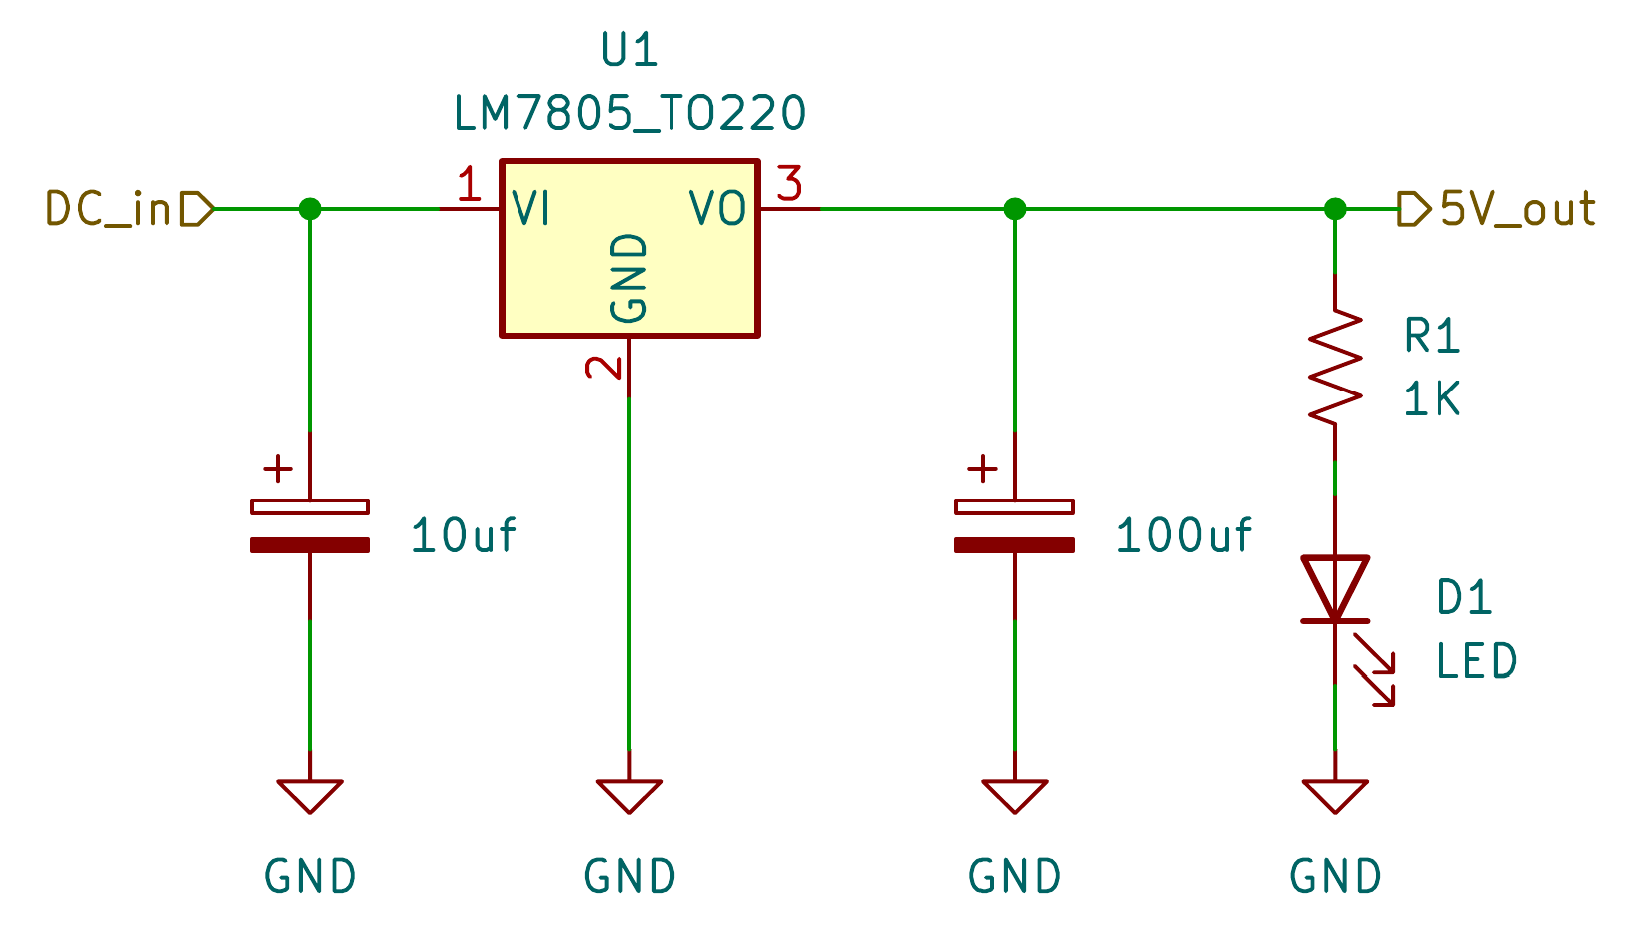
\includegraphics[width=0.5\textwidth]{image/fuente.png}
    \caption{Fuente de alimentación}\label{fig:fuente}
\end{figure}

En la Figura~\ref{fig:fuente} se muestra el circuito esquemático de la fuente de alimentación.

El circuito puede alimentarse tanto desde una fuente de tensión continua externa, como desde una batería de 9V.
Para esto, el circuito cuenta con una llave que permite seleccionar la fuente de alimentación deseada,

\begin{figure}[H]
    \centering
    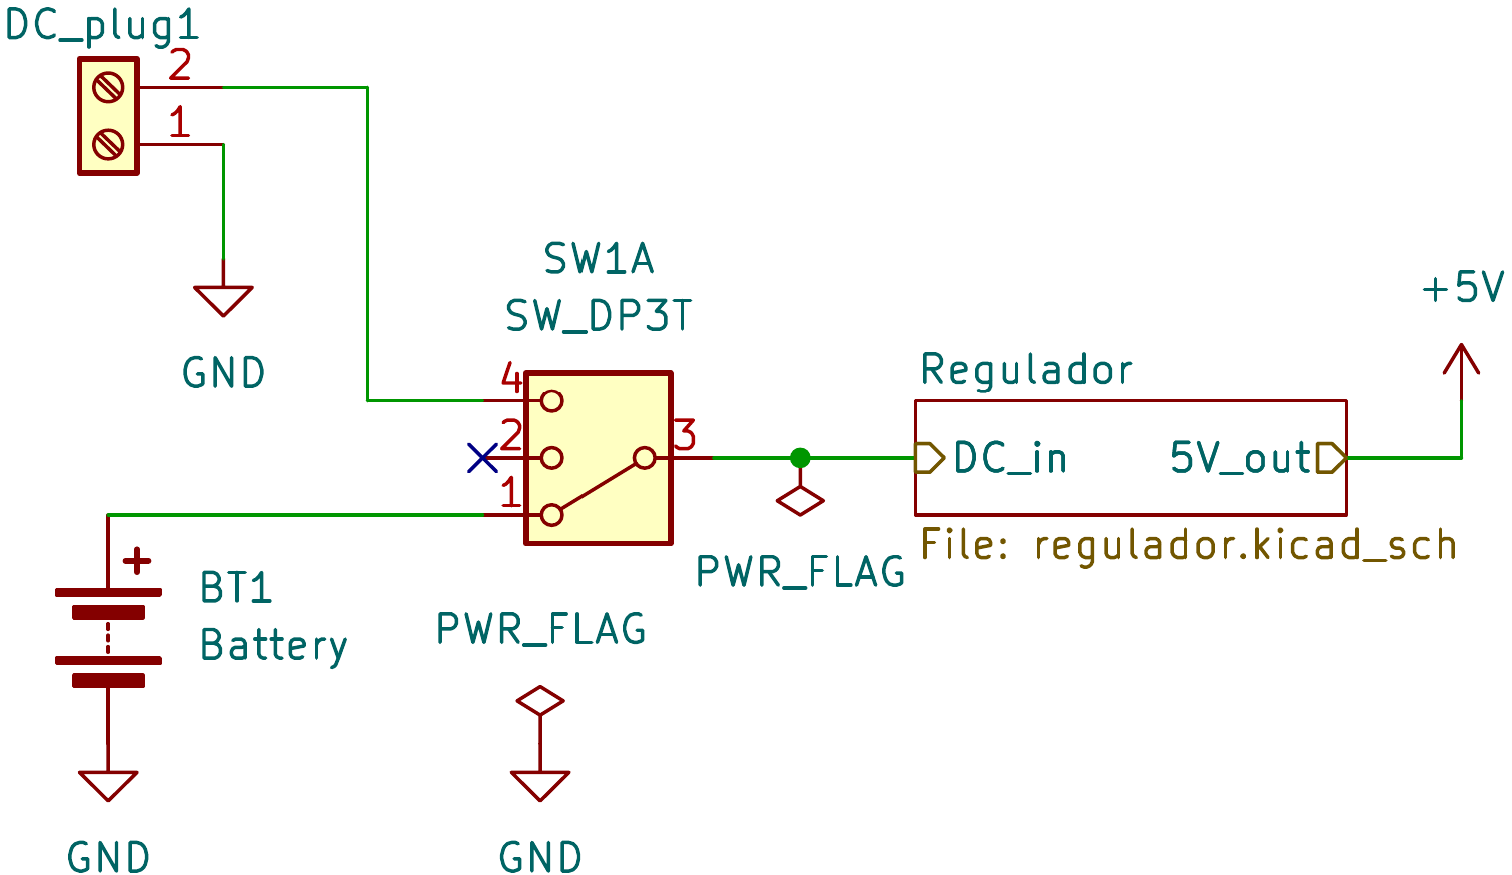
\includegraphics[width=0.5\textwidth]{image/selector.png}
    \caption{Selector de fuente de alimentación}\label{fig:selector}
\end{figure}

\subsubsection{Bloque de Salidas Digitales}
Este bloque consta de 6 salidas digitales, cada una de las cuales puede proporcionar un nivel lógico alto o bajo.
Estas salidas se utilizan para simular distintas combinaciones de entrada en los circuitos lógicos que se deseen probar.
El estado de cada salida se selecciona mediante una llave.
Además, cada salida cuenta con un LED indicador que muestra su estado actual, lo que facilita la visualización de las combinaciones lógicas.
Cada una de estas salidas se expone a través de una bornera para su conexión al circuito en prueba.

\begin{figure}[H]
    \centering
    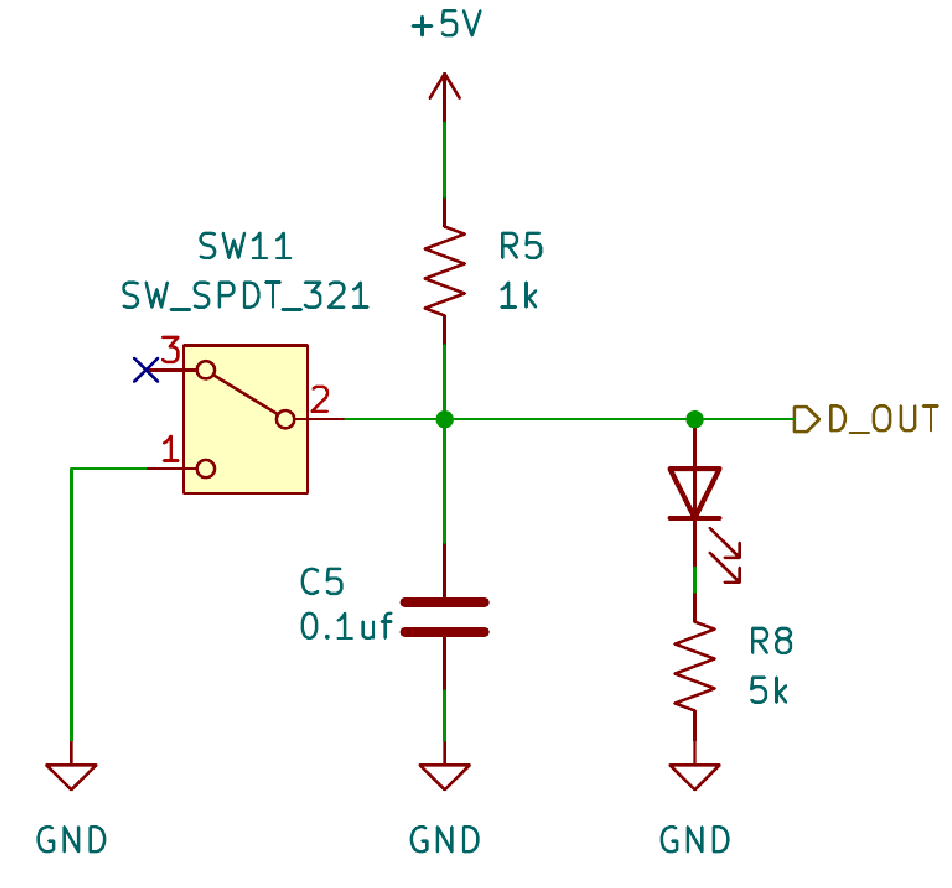
\includegraphics[width=0.3\textwidth]{image/salida.png}
    \caption{Salida digital}\label{fig:salida}
\end{figure}

En la Figura~\ref{fig:salida} se muestra el circuito esquemático de una salida digital.

\subsubsection{Bloque de Entradas Digitales}
Este bloque incluye 6 entradas digitales.
Cada entrada está asociada a un LED indicador que refleja su estado lógico:
\begin{itemize}
    \item LED apagado: lógico “0”
    \item LED encendido: lógico “1”
\end{itemize}
Esto permite verificar visualmente el estado de cada una.
Cada una de estas entradas se expone a través de una bornera para su conexión al circuito en prueba.

\begin{figure}[H]
    \centering
    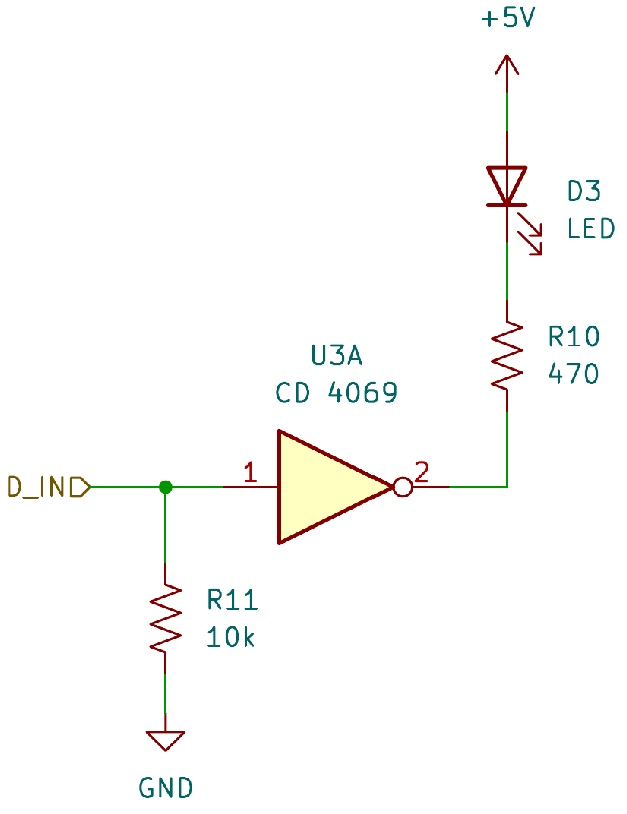
\includegraphics[width=0.3\textwidth]{image/entrada.png}
    \caption{Entrada digital}\label{fig:entrada}
\end{figure}

En la Figura~\ref{fig:entrada} se muestra el circuito esquemático de una entrada digital.

\subsubsection{Bloque de Generador de Señal}
Este bloque consiste en un generador de señal de onda cuadrada, implementado mediante un temporizador 555 configurado en modo astable.
La frecuencia de la señal generada es ajustable mediante un potenciómetro.
Esta señal será utilizada como señal de clock para ensayas circuitos secuenciales.
Se incluyó un LED indicador que parpadea al ritmo de la señal generada.
La señal de salida se expone a través de una bornera para su conexión al circuito en prueba.

\begin{figure}[H]
    \centering
    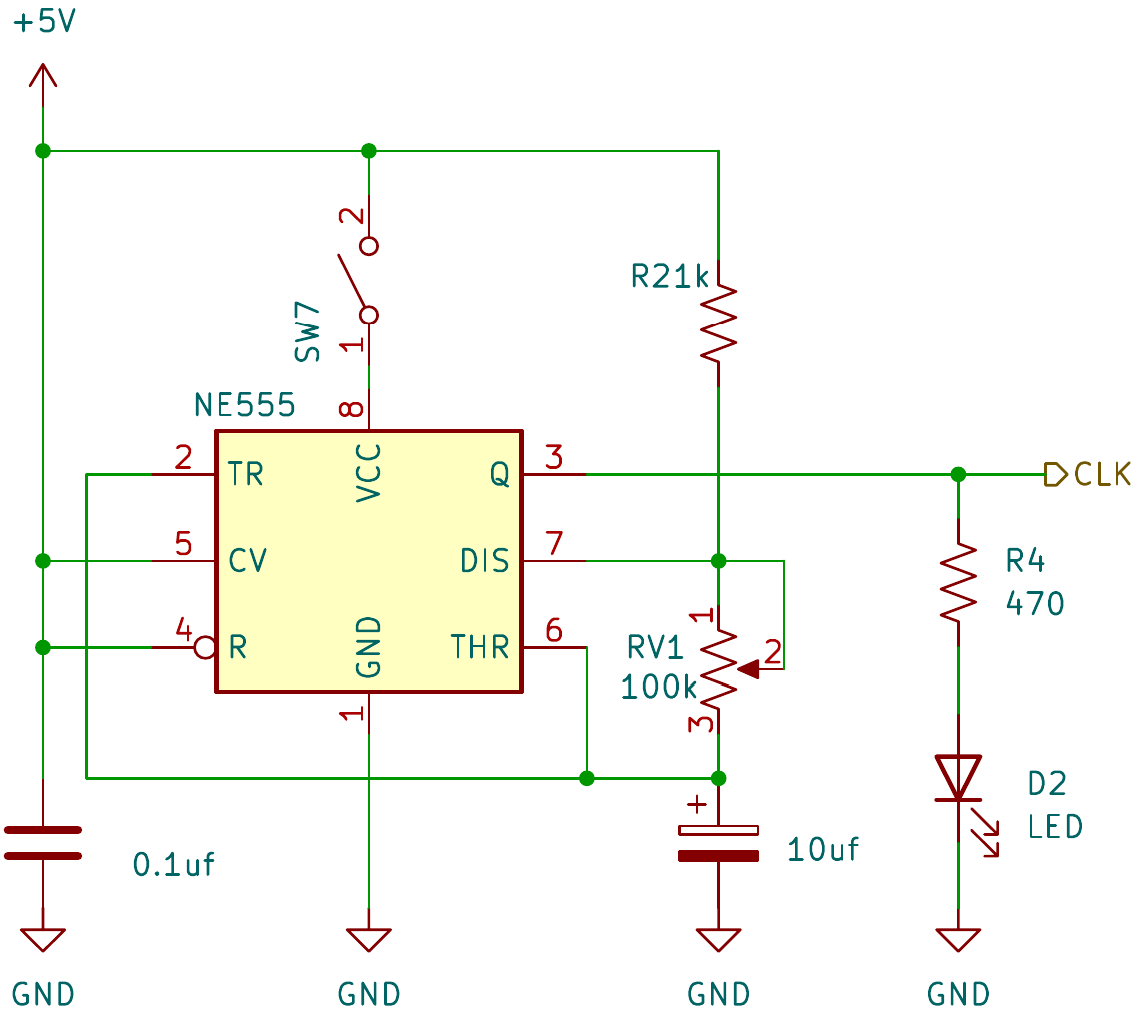
\includegraphics[width=0.5\textwidth]{image/generador.png}
    \caption{Generador de señal}\label{fig:generador}
\end{figure}

En la Figura~\ref{fig:generador} se muestra el circuito esquemático del generador de señal.

\subsection{Circuito implementado}

%\textit{Incluir el esquema o una imagen del circuito armado.}
El circuito esquemático completo del MiniLab se encuentra en el anexo~\ref{anexo:circuito} al final del informe.
En la figura~\ref{fig:implementacion} se muestra una imagen del circuito implementado.

\begin{figure}[H]
    \centering
    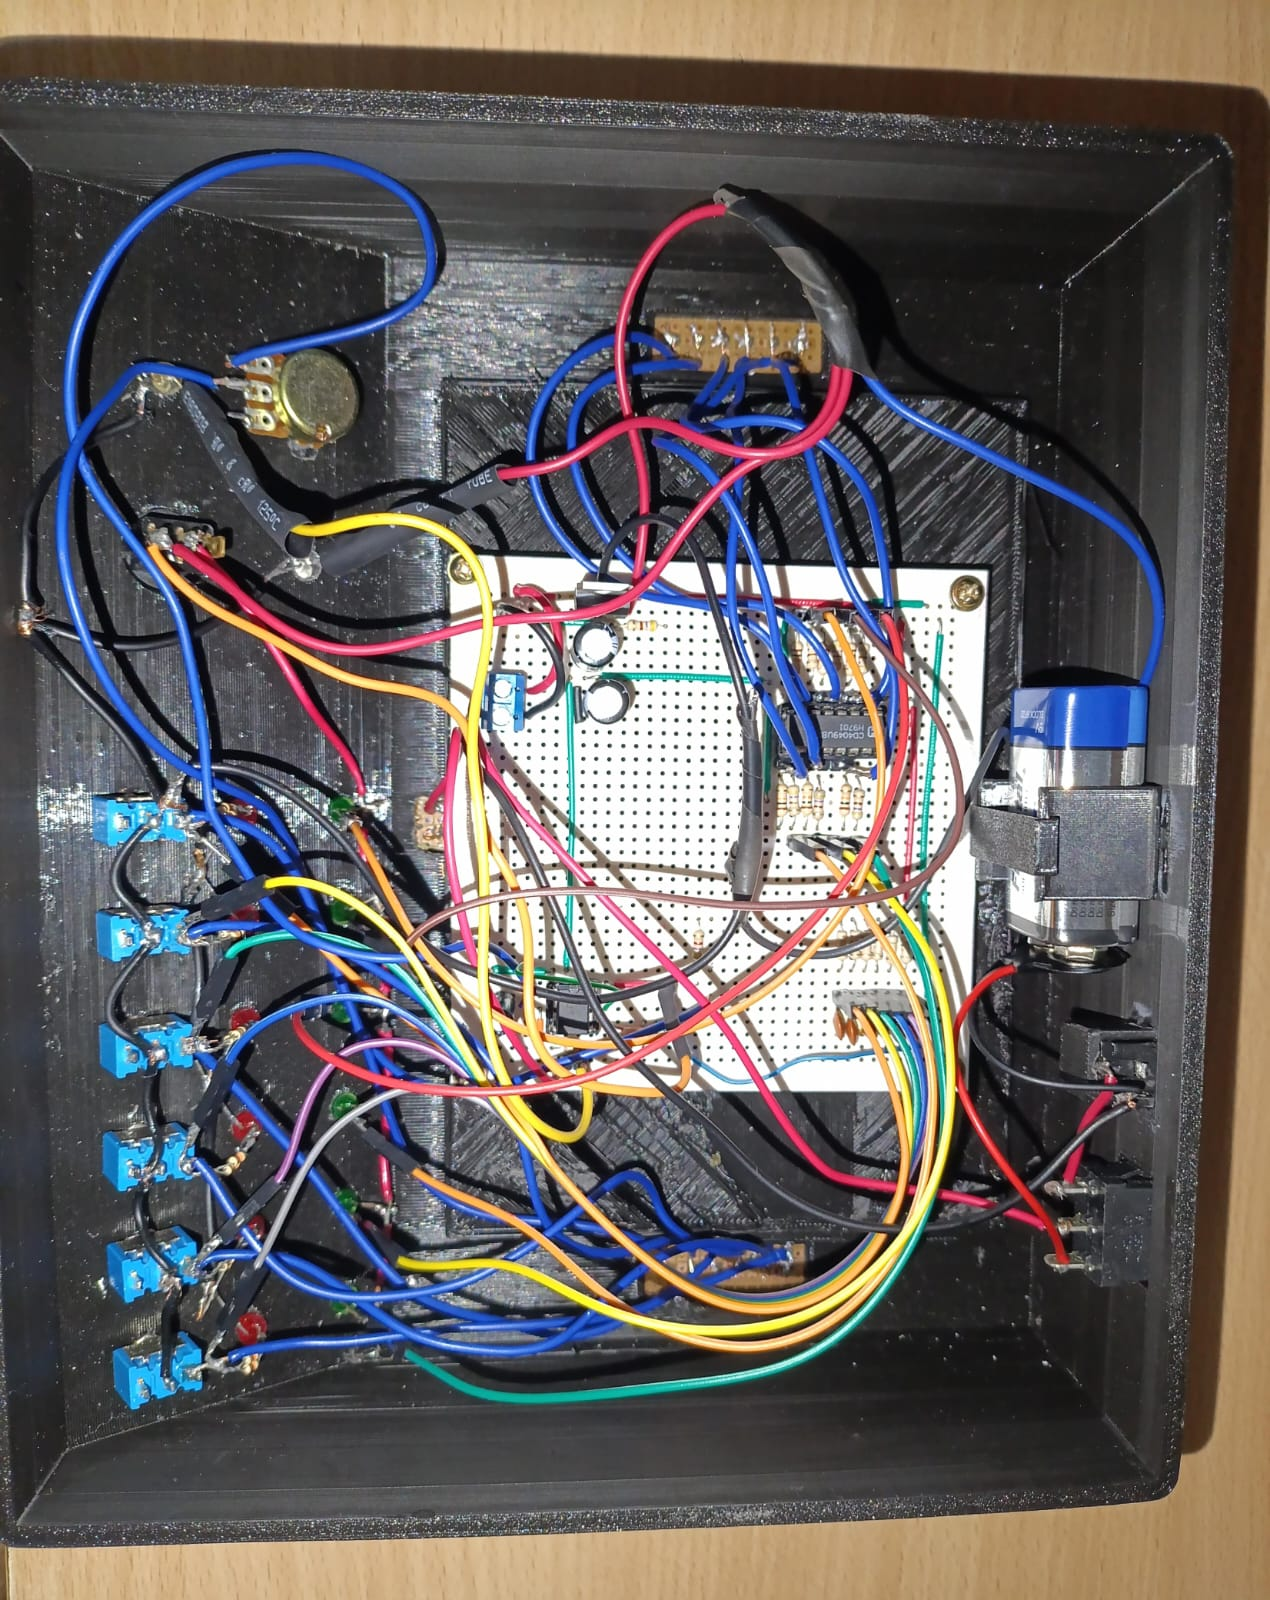
\includegraphics[width=0.5\textwidth]{image/implementacion.jpeg}
    \caption{Circuito implementado en el MiniLab}\label{fig:implementacion}
\end{figure}

\subsection{Funcionamiento}
El MiniLab está diseñado de forma que permite alimentar, generar señales de reloj, y establecer entradas y salidas para
probar circuitos digitales. A continuación se describe el flujo de funcionamiento general y cómo interactúan los distintos bloques.

Primero, la alimentación se selecciona mediante el selector mostrado en la Figura~\ref{fig:selector}. Se puede elegir
entre la alimentación desde una fuente de continua externa o una batería de 9V interna. La tensión seleccionada
entra al regulador LM7805, que proporciona una salida estable de 5V para todo el sistema. Un LED indicador muestra
cuando la alimentación está presente.

Las salidas digitales permiten generar niveles lógicos `0` (0V) y `1` (5V) para aplicar a un circuito
en prueba. Cada salida está controlada por una llave que selecciona el estado lógico y dispone de un LED indicador que
refleja visualmente el nivel aplicado (Figura~\ref{fig:salida}). Las salidas se exponen mediante borneras para
facilitar la conexión.

Las entradas digitales están pensadas para recibir señales externas desde el circuito bajo prueba. Cada entrada
incluye un LED indicador que permanece apagado para nivel lógico `0` y encendido para nivel lógico `1`
(Figura~\ref{fig:entrada}).

El generador de señal implementado con un temporizador 555 en configuración astable provee una onda cuadrada cuyo
periodo se ajusta mediante un potenciómetro. La frecuencia ajustable (aproximadamente 1 Hz a 1 kHz) se utiliza como
reloj para ensayar circuitos secuenciales; un LED adicional parpadea sincronizado con la señal generada
(Figura~\ref{fig:generador}).

Modo de uso típico:
\begin{enumerate}
    \item Seleccionar la fuente de alimentación adecuada y encender el MiniLab.
    \item Configurar las salidas mediante sus llaves para aplicar los niveles lógicos deseados al circuito en prueba.
    \item Si se requiere una señal de reloj, ajustar la frecuencia del generador y conectar su salida al pin de clock del circuito en prueba.
    \item Conectar las entradas a los puntos de medida del circuito; observar los LEDs de entrada para verificar estados lógicos y analizar
        el funcionamiento del circuito en prueba.
\end{enumerate}

%--------------------------------
\section{Resultados}
%--------------------------------

% \textit{Describir qué resultados se obtuvieron. Indicar si el sistema funciona correctamente.}
En la Figura~\ref{fig:resultados} se muestra el funcionamiento del MiniLab, conectando las entradas con las salidas y
verificando el estado de los LEDs indicadores.
Los LEDs rojos indican el estado de las salidas digitales, mientras que los LEDs verdes muestran el estado de las entradas digitales.

\begin{figure}[H]
    \centering
    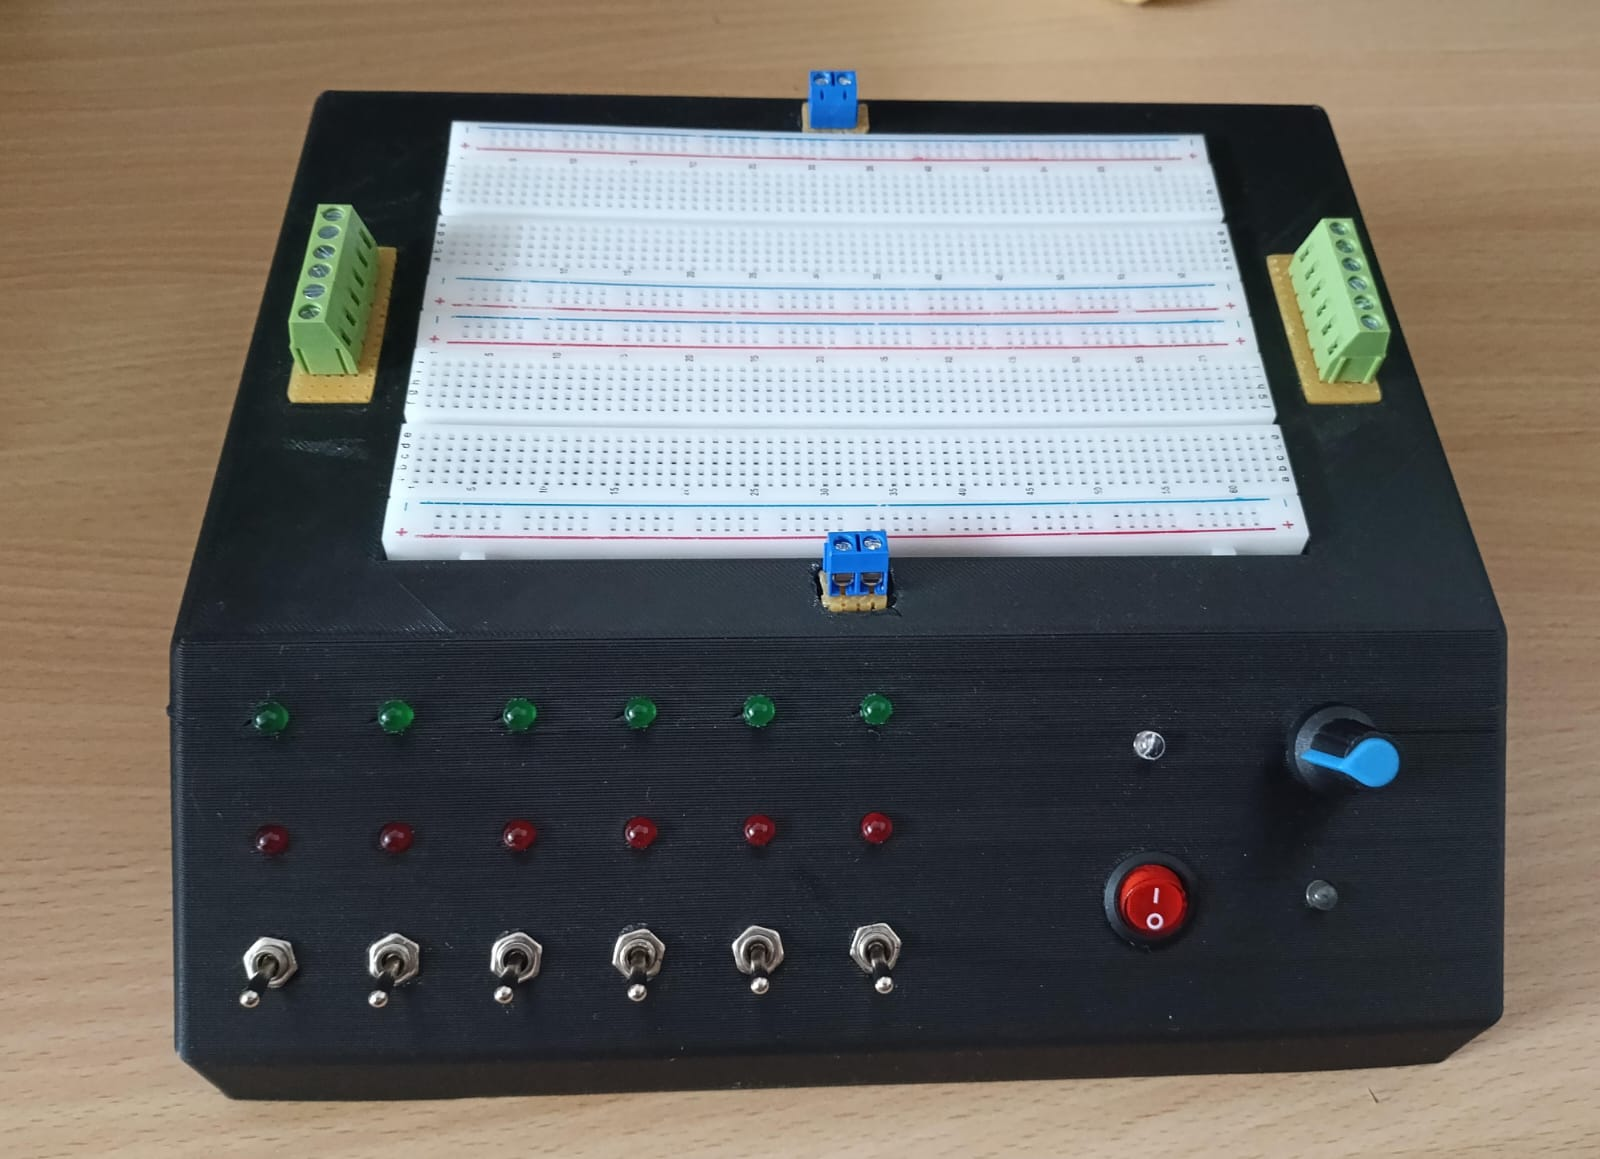
\includegraphics[width=0.6\textwidth]{image/resultados.jpeg}
    \caption{Resultados obtenidos al probar el MiniLab}\label{fig:resultados}
\end{figure}

En la Figura~\ref{fig:resultados} se puede observar que el sistema funciona correctamente, ya que al conectar las entradas con las salidas,
los LEDs indicadores reflejan el estado lógico de las entradas y salidas según lo esperado.

\subsection{Requerimientos no alcanzados}
\textbf{Tensión de salida para el nivel alto:} El nivel lógico alto se estableció en 4.45V en lugar de los 5V requeridos. Esto
es debido a la incorporación del LED indicador. Sin embargo, este nivel de tensión está dentro del rango considerado como lógico alto
tanto para TTL(>2V) como para CMOS (>3.5V), por lo que no afecta el funcionamiento del sistema.

%--------------------------------
\section{Dificultades encontradas}
%--------------------------------

%\textit{Mencionar problemas durante el armado y cómo fueron resueltos.}
La mayor dificultad encontrada durante el armado del MiniLab fue la combinación de resistencia y capacidad 
para obtener la frecuencia deseada en el generador de señal basado en el temporizador 555. Para resolver este problema,
se realizaron cálculos teóricos utilizando las fórmulas provistas por el fabricante para determinar los valores adecuados
de resistencia y capacidad, y luego se realizaron pruebas prácticas ajustando estos componentes hasta alcanzar la frecuencia deseada.

Por fuera de esto, durante el armado del MiniLab no encontramos dificultades significativas. Las tareas fueron distribuidas entre los
integrantes del grupo, lo que permitió avanzar de manera fluida en el proceso de construcción. A la hora de integrar 
el trabajo de cada integrante no hubo inconvenientes ya que se mantuvo un buen nivel de comunicación y coordinación entre todos.

%--------------------------------
\section{Conclusión}
%--------------------------------
El MiliLab construido cumple con los requerimientos funcionales establecidos, proporcionando una herramienta práctica
para la experimentación con circuitos digitales.

La construcción del MiniLab nos permitió desarrollar habilidades de interpretación de circuitos esquemáticos, lectura
e interpretación de hojas de datos del fabricante, manejo de herramientas de laboratorio, y habilidades prácticas en
el armado y verificación de circuitos electrónicos.

A través de este proyecto, comprendimos la importancia de una buena planificación y distribución de tareas para lograr un resultado exitoso. 

%--------------------------------
\section{Anexos}
%--------------------------------
\subsection{Circuito esquemático}\label{anexo:circuito}

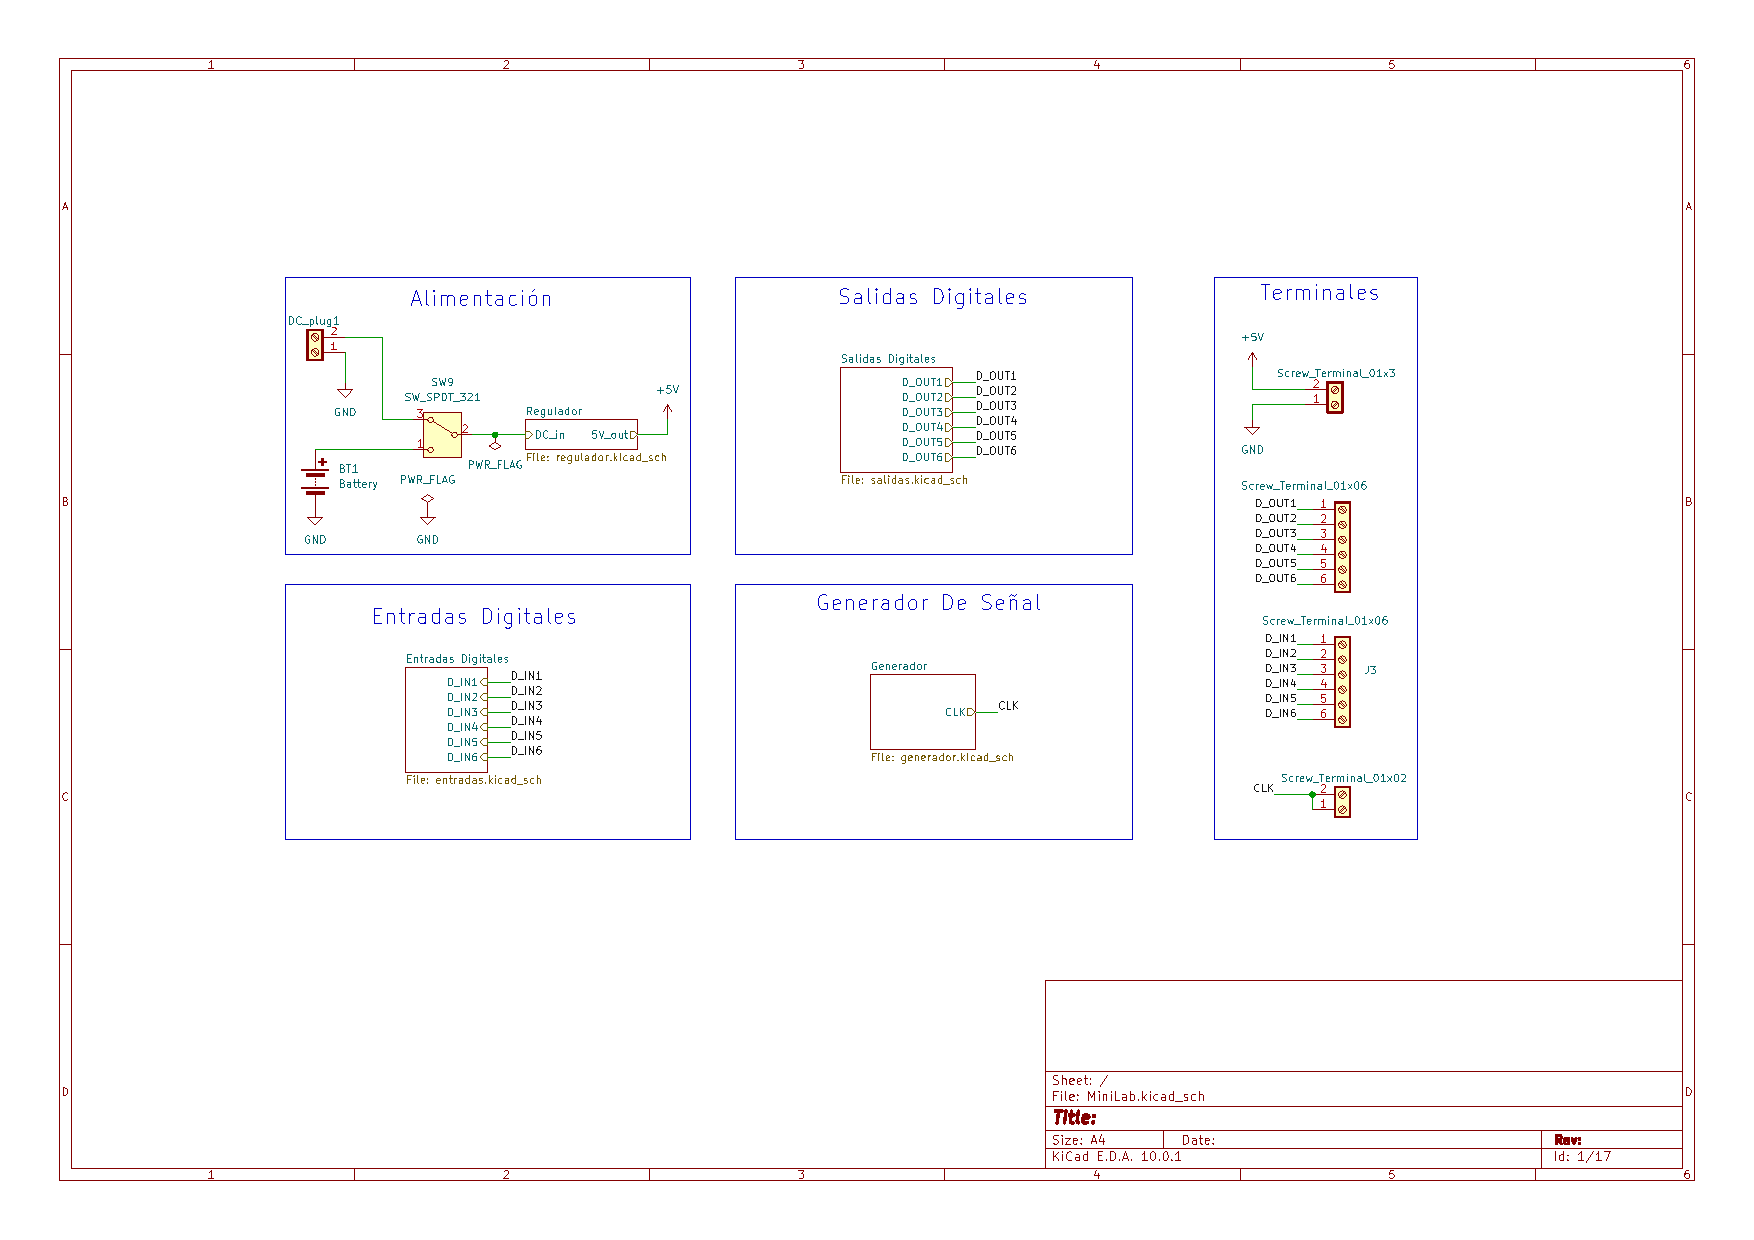
\includepdf[pages=-, landscape=true]{../sch/output.pdf}

\end{document}

